\documentclass[12pt]{amsart}
\usepackage[margin=1in]{geometry}

\usepackage{tikz}
\usetikzlibrary{positioning}

\usepackage{amsmath,amsfonts,amssymb,amsthm}
\usepackage{enumitem}
\usepackage{colonequals,multicol}
\usepackage{xcolor}
\usepackage{fancyhdr}
%\usepackage{cleveref}
\usepackage{hyperref}

\newcommand{\Q}{\mathbb{Q}}
\newcommand{\N}{\mathbb{N}}
\newcommand{\Z}{\mathbb{Z}}
\newcommand{\R}{\mathbb{R}}
\DeclareMathOperator{\im}{image}
\DeclareMathOperator{\id}{id}


\theoremstyle{definition} 
\newtheorem*{definition}{Definition}
\newtheorem*{example}{Example}
\newtheorem{theorem}{Theorem}
\newtheorem{lemma}{Lemma}
\newtheorem{corollary}{Corollary}
\newtheorem{proposition}{Proposition}
\newtheorem{statement}{Statement}
\newtheorem*{remark}{Remark}



\begin{document}
	
\thispagestyle{fancy}
\pagestyle{fancy}
\lhead{\scriptsize University \textit{of} Nebraska-Lincoln}
\rhead{\scriptsize Math of Machine Learning}
\chead{Worksheet 5}
	
	\
 
\begin{center}
    {\Large \bf {\sc Backpropagation}}
\end{center}

\

\textit{Backpropagation} is an algorithm for computing the gradient of a loss function for an~ANN. \\

\noindent \textbf{Chain Rule:} For the composition of functions $f(x) = (f_1 \circ f_{2} \circ \cdots \circ f_{n-1} \circ f_n) (x)$,
    \[
        \frac{df}{dx} = \frac{df_1}{df_2} \frac{df_2}{df_3} \cdots \frac{df_{n-1}}{df_n} \frac{df_n}{dx}
    \]

\vspace{.5em}
\begin{enumerate}[itemsep=2.5em,leftmargin=0pt]
%%%%%%%%%%%%%%%%%%%%%%%%%%%%%%%%%%%%%%%%

\item Let $f = 4f_1^2$, $f_1=f_2-2$, $f_2 = 5x^3 - x + 1$. Use the chain rule to compute $\frac{df}{dx}$.

\vspace{2.5em}
%%%%%%%%%%%%%%%%%%%%%%%%%%%%%%%%%%%%%%%%

\noindent Recall the chain rule with partial derivatives:\vspace{.5em}

\noindent \textbf{Chain Rule with Partial Derivatives} Let us assume $z= f(x,y)$ and that both $x$ and $y$ are functions of other variables $u, v$, i.e $x= x(u,v), y= y(u,v)$. Then we can define $\frac{\partial f}{\partial u}, \frac{\partial f}{\partial v}$ using chain rule,
        $$\frac{\partial f}{\partial u} = \frac{\partial f}{\partial x} \frac{\partial x}{\partial u}+ \frac{\partial f}{\partial y} \frac{\partial y}{\partial u}, \quad  \frac{\partial f}{\partial v} = \frac{\partial f}{\partial x} \frac{\partial x}{\partial v}+ \frac{\partial f}{\partial y} \frac{\partial y}{\partial v}$$

\noindent More generally, if $z=f(x_1,x_2,\ldots,x_n)$ and each $x_i$ are a function of $u, v$, then 
    $$ \frac{\partial f}{\partial u} = \sum_{k=1}^n \frac{\partial f}{\partial x_k} \frac{\partial x_k}{\partial u}$$
Similarly for $\frac{\partial f}{\partial v}$.

\vspace{-1.5em}
%%%%%%%%%%%%%%%%%%%%%%%%%%%%%%%%%%%%%%%%

\item Suppose $f(x,y) = 2x^3 + y$, $x(u,v)=\sin(u)+\cos(v)$, and $y(u,v)=e^{uv}$. Compute $\frac{\partial f}{\partial u}$ and $\frac{\partial f}{\partial v}$.

\vspace{2.5em}
%%%%%%%%%%%%%%%%%%%%%%%%%%%%%%%%%%%%%%%%

\noindent Remember that an FNN is a sequence of compositions of linear transformations and non-linear functions. The chain rule is the most important ingredient for computing the gradients of a given loss function for the weights of an FNN. \\

\noindent \textbf{Notation:} Define the weight from the $k^{\text{th}}$ neuron in the $(l-1)^{\text{th}}$ layer to the $j^{\text{th}}$ neuron in the $l^{\text{th}}$ layer as $w^l_{jk}$. Similarly, we denote by $b^l_j$ the $j^{\text{th}}$ bias in the $l^{\text{th}}$ layer, $a^l_j$ the $j^{\text{th}}$ activated neuron in the $l^{\text{th}}$ layer (after applying the activation function), and $z^l_j$ the $j^{\text{th}}$ pre-activated neuron (before applying the activation function).
\begin{figure}[h!]
    \centering
    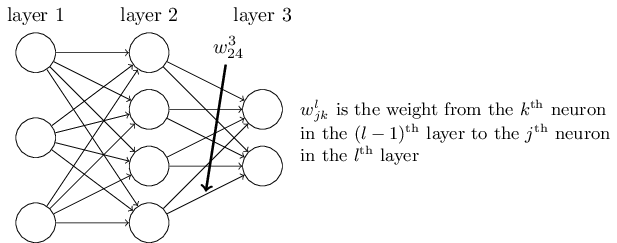
\includegraphics[width=0.75\linewidth]{figures/tikz16.png}
    \caption{Image from Michael Nielsen's \href{http://neuralnetworksanddeeplearning.com/index.html}{\textit{Neural Networks and Deep Learning}}.}
    \label{fig:weight-notation}
\end{figure}

\vspace{-1.5em}
%%%%%%%%%%%%%%%%%%%%%%%%%%%%%%%%%%%%%%%%

\item Write out the labels of each neuron in Figure~\ref{fig:weight-notation} using the notation $a^l_j$.

\vspace{2.5em}
%%%%%%%%%%%%%%%%%%%%%%%%%%%%%%%%%%%%%%%%

\noindent Let $\sigma$ be an activation function. With this notation,
\begin{equation}\label{eq:neuron}
    a^l_j = \sigma\left( z^l_j \right), \qquad 
    z^l_j = \sum_k w^l_{jk}a^{l-1}_k +b^l_j, \qquad
\end{equation}

\noindent Each layer of a FNN represents a vector. To get from one layer to the next, we compute $\sigma(W\mathbf{a}+\mathbf{b})$ where $\sigma$ is an activation function, $W$ is a matrix, $\bf a$ is a vector representing the previous layer, and $\bf b$ is a bias vector. For consistency of notation, use $W^l$ and ${\bf b}^l$ to represent the matrix and biases that maps the $(l-1)^{\text{th}}$ layer ${\bf a}^{l-1}$ to the $l^{\text{th}}$ layer ${\bf a}^l$. Hence,
\begin{equation}\label{eq:layer}
    {\bf a}^l = \sigma\left( {\bf z}^l \right), \qquad
    {\bf z}^l = W^{l} {\bf a}^{l-1} + {\bf b}^{l}
\end{equation}

\vspace{-1.5em}
%%%%%%%%%%%%%%%%%%%%%%%%%%%%%%%%%%%%%%%%

\item Consider the FNN in Figure~\ref{fig:weight-notation}. Write out the matrices $W^l$ and bias vectors ${\bf b}^l$ for $l=2,3$ using the notation for the weights $w^l_{jk}$ and biases $b^l_j$.

\item Briefly explain how the equations for $a^l_j$ and $z^l_j$ in Equation~\ref{eq:neuron} are derived from Equation~\ref{eq:layer}. 

\vspace{2.5em}
%%%%%%%%%%%%%%%%%%%%%%%%%%%%%%%%%%%%%%%% 

\noindent \textbf{Goal:} Compute the gradient vector of a loss function $L$ for any weights and biases. That is, we must compute 
    \[ \frac{\partial L}{\partial w^l_{jk}} \qquad \text{and} \qquad \frac{\partial L}{\partial b^l_{j}} \] 
for all~$l,j,k$. \\

\noindent Before we do this, let's do a couple more problems and define an operation that will be useful for programming backpropagation.

\vspace{-1.5em}
%%%%%%%%%%%%%%%%%%%%%%%%%%%%%%%%%%%%%%%%

\item Compute $\displaystyle \frac{\partial z^l_j}{w^l_{jk}}$ and $\displaystyle \frac{\partial z^l_j}{b^l_{j}}$.

\vspace{2em}
%%%%%%%%%%%%%%%%%%%%%%%%%%%%%%%%%%%%%%%%

\begin{definition}The \textbf{Hadamard product} denoted by $\odot$ is the element-wise product of two vectors of the same size. That is,
    \[
        \begin{bmatrix} x_1\\ x_2 \\ \vdots \\ x_n \end{bmatrix}
            \odot
        \begin{bmatrix} y_1\\ y_2 \\ \vdots \\ y_n \end{bmatrix}
        = \begin{bmatrix} x_1y_1\\ x_2y_2 \\ \vdots \\ x_ny_n \end{bmatrix}
    \]
\end{definition}

\vspace{-1.5em}
%%%%%%%%%%%%%%%%%%%%%%%%%%%%%%%%%%%%%%%%

\item Compute 
    \(
        \begin{bmatrix} 0\\ 1 \\ 5 \\ 2 \end{bmatrix}
            \odot
        \begin{bmatrix} 3\\ 2 \\ 1 \\ 9 \end{bmatrix}
    \)

\vspace{2.5em}
%%%%%%%%%%%%%%%%%%%%%%%%%%%%%%%%%%%%%%%%

\noindent Pause to derive the following equations with the whole class for backpropagation:
\begin{align*}
    {\bf d}^F &= \nabla_a L \odot \sigma'\left({\bf z}^F\right),  & 
        d^F_j &= \frac{\partial L}{\partial a^F_j} \sigma'(z^F_j)  \\
    {\bf d}^l &= \left( \left( W^{l+1} \right)^T {\bf d}^{l+1} \right) \odot \sigma'\left({\bf z}^l\right),  &
        d^l_j &= \sum_k w^{l+1}_{kj} d^{l+1}_k \sigma'\left(z^l\right) \\
    \frac{\partial L}{\partial w^l_{jk}} &= a^{l-1}_k d^l_j \\
    \frac{\partial L}{\partial b^l_j} &= d^l_j
\end{align*}
where $F$ is the number of layers (i.e., layer~$F$ is the final layer), $\displaystyle d^l_j = \frac{\partial L}{\partial z^l_j}$, $\mathbf{d}^l = \left[d^l_1, d^l_2, \ldots, d^l_{n} \right]^T$, and $n$ is the number of nodes in the $l^{\text{th}}$ layer. \\ ~ \\

\noindent \underline{\textbf{Backpropagation Algorithm}} \\
\begin{enumerate}[label=\arabic*.,itemsep=1em]
    \item \textbf{Input $x$:} Set the corresponding activation ${\bf a}^1$ for the input layer.
    \item \textbf{Feedforward:} For each $l=2,3,\ldots, F$ compute ${\bf z}^l = W^l {\bf a}^{l-1} + {\bf b}^l$ and ${\bf a}^l = \sigma\left({\bf z}^l\right)$.
    \item \textbf{Output ${\bf d}^F$:} Compute ${\bf d}^F=\nabla_a L \odot \sigma'\left({\bf z}^F\right)$.
    \item \textbf{Backpropagate:} For each $l=L-1,L-2,\ldots,2$ compute ${\bf d}^l = \left( \left( W^{l+1} \right)^T {\bf d}^{l+1} \right) \odot \sigma'\left({\bf z}^l\right)$.
    \item \textbf{Output}: The gradient of the cost function is given by $\displaystyle \frac{\partial L}{\partial w^l_{jk}} = a^{l-1}_k d^l_j$ and $\displaystyle \frac{\partial L}{\partial b^l_j} = d^l_j$.
\end{enumerate}

\noindent \textbf{Total Loss:} At this point, everything we've done to compute the partials $\displaystyle \frac{\partial L}{\partial w^l_{jk}}$ and $\displaystyle \frac{\partial L}{\partial b^l_j}$ for a single input ${\bf a}^1$. Suppose we have $n$ training samples. Then the total loss function is given by 
    $$ L_{T} = \frac{1}{n}\sum_{i=1}^n L_i 
    = \frac{1}{n}\sum_{i=1}^n L\left( {\bf y}_i, \tilde{{\bf y}}_i \right) 
    = \frac{1}{n}\sum_{i=1}^n L\left( {\bf y}_i, {\bf a}^F_i \right), $$
where ${\bf y}_i$ is the true value and $\tilde{{\bf y}}_i={\bf a}^F_i$ is the predicted value given by the final layer for each input.

%%%%%%%%%%%%%%%%%%%%%%%%%%%%%%%%%%%%%%%%

\item Compute $\displaystyle \frac{\partial L_T}{\partial w^l_{jk}}$ and $\displaystyle \frac{\partial L_T}{\partial b^l_{j}}$ with respect to $\displaystyle \frac{\partial L_i}{\partial w^l_{jk}}$ and $\displaystyle \frac{\partial L_i}{\partial b^l_{j}}$.

\vspace{2.5em}
%%%%%%%%%%%%%%%%%%%%%%%%%%%%%%%%%%%%%%%%

\noindent \textbf{Note:} To perform gradient descent, we use $\displaystyle \frac{\partial L_T}{\partial w^l_{jk}}$ and $\displaystyle \frac{\partial L_T}{\partial b^l_{j}}$ to update the model weights and biases. To perform stochastic gradient descent, we change the total loss to the batch loss $L_B$ which is defined similarly to total loss but for a specific batch of our training dataset instead of all of it.

%%%%%%%%%%%%%%%%%%%%%%%%%%%%%%%%%%%%%%%%

\item Let $\sigma$ be the sigmoid activation function. Compute $\sigma'$.

\item Let $\sigma$ be the ReLU activation function. Compute $\sigma'$. \textit{Hint:} Your answer should be a piecewise function.

\item Let $L$ be the mean squared error loss function. Compute $\nabla_a L$. That is, compute $\displaystyle \frac{\partial L}{\partial a^F_j}$ for all nodes $j$ in the final layer.

\end{enumerate}

\end{document}